\documentclass[a4paper]{article}
\usepackage{graphicx}
\usepackage{fullpage}
\usepackage{graphicx} % for pdf, bitmapped graphics files
\usepackage{amsmath} % assumes amsmath package installed
\usepackage{amssymb}  % assumes amsmath package installed\ref
\usepackage{psfrag}
\usepackage{algorithmic}
\usepackage{algorithm}
\usepackage{color}
\usepackage{xcolor}
\usepackage{listings}
\usepackage[T1]{fontenc}
\begin{document}

\lstset{
language=C++,
captionpos=b,
tabsize=2,
keywordstyle=\color{blue},
commentstyle=\color{green},
stringstyle=\color{red},
breaklines=true,
showstringspaces=false,
frame=shadowbox,
rulesepcolor=\color{gray},
basicstyle=\footnotesize%
}


\newcommand{\gopt}{g\ensuremath{^2}o}
\newcommand{\defeq}{\stackrel{\text{def.}}{=}}
\newcommand{\gcomment}[1]{\textcolor{red}{\textbf{Giorgio:}~\emph{#1}}}
\newcommand{\rcomment}[1]{\textcolor{red}{\textbf{Rainer:}~\emph{#1}}}

\def\secref#1{Section~\ref{#1}}
\def\figref#1{Figure~\ref{#1}}
\def\tabref#1{Table~\ref{#1}}
\def\eqref#1{Eq.~\ref{#1}}

\newcommand{\Dom}{\mathtt{Dom}}
\newcommand{\bZero}{\mathbf{0}}
\newcommand{\bb}{\mathbf{b}}
\newcommand{\bc}{\mathbf{c}}
\newcommand{\bh}{\mathbf{h}}
\newcommand{\bH}{\mathbf{H}}
\newcommand{\bA}{\mathbf{A}}
\newcommand{\bM}{\mathbf{M}}
\newcommand{\bF}{\mathbf{F}}
\newcommand{\bG}{\mathbf{G}}
\newcommand{\bI}{\mathbf{I}}
\newcommand{\bB}{\mathbf{B}}
\newcommand{\bR}{\mathbf{R}}
\newcommand{\bp}{\mathbf{p}}
\newcommand{\bq}{\mathbf{q}}
\newcommand{\bqTilde}{\mathbf{\tilde q}}
\newcommand{\ec}{\mathbf{e}}
\newcommand{\be}{\mathbf{e}}
\newcommand{\br}{\mathbf{r}}
\newcommand{\bx}{\mathbf{x}}
\newcommand\bbx{\breve{\bx}}
\newcommand{\bu}{\mathbf{u}}
\newcommand{\bz}{\mathbf{z}}
\newcommand{\bt}{\mathbf{t}}
\newcommand{\bDeltax}{\mathbf{\Delta x}}
\newcommand{\bDeltaAlpha}{\mathbf{\Delta \alpha}}
\newcommand{\bDeltaAlphaTilde}{\mathbf{\Delta\tilde\alpha}}
\newcommand{\bTDeltax}{\mathbf{\Delta \tilde x}}
\newcommand{\bDelta}{\mathbf{\Delta}}
\newcommand{\balpha}{\mathbf{\alpha}}
\newcommand{\bOmega}{\mathbf{\Omega}}
\newcommand{\bSigma}{\mathbf{\Sigma}}
\newcommand{\bJ}{\mathbf{J}}
\newcommand{\diff}{\partial}
\def\argmax{\mathop{\rm argmax}}
\def\argmin{\mathop{\rm argmin}}

\newcommand{\Rstar}{{\cal R} }
\newcommand{\Rx}{R}
\newcommand{\tx}{t}

\newcommand{\angleOf}{\mathbf{angleOf}}
\newcommand{\axisOf}{\mathbf{axisOf}}
\newcommand{\slerp}{\mathbf{slerp}}

\title{Lane Quality Assessment for Autonomous Driving}
\author{
	Binbin~Li\thanks{B. Li and D. Song are with Department of Computer Science and Engineering, Texas A\&M University, College Station, TX, 77843, US. (email: {\tt\footnotesize {binbinli@tamu.edu}, dzsong@cse.tamu.edu})}, 
	Dezhen~Song\footnotemark[1], 
	Haifeng Li\thanks{H. Li is with Computer Science Department, Civil Aviation University of China, Tianjin, 300300, China, and also with Fujian Provincial Key Laboratory of Information Processing and Intelligent Control, Minjiang University, Fuzhou, 350108, China. (email:{\tt\footnotesize hfli@cauc.edu.cn})}, 
	Adam Pike\thanks{A. Pike is with Texas A\&M Transportation Institute, College Station, TX, 77843, US. (email: {\tt\footnotesize A-Pike@tti.tamu.edu})}, 
	and Paul Carlson\thanks{P. Carlson is with Road Infrastructure, Inc., College Station, TX, 77843, US. (email: {\tt\footnotesize  PCarlson@roadinfrastructureinc.com}) }
%	email: \texttt{binbinli@tamu.edu dzsong@cse.tamu.edu  hfli@cauc.edu.cn}\\
%        \texttt{A-Pike@tti.tamu.edu PCarlson@roadinfrastructureinc.com}
}



\maketitle

We describe a C++ framework to quantify the lane quality to assist autonomous driving in urban scenarios. We propose different metrics and and algorithms by detecting and tracking immediate left and right lane boundaries with respect to the vehicle due to their importance in guiding the vehicle. We do not identify multiple parallel lanes simultaneously because the onboard sensors have perspective limitations. 

The vehicle is equipped with one front view camera, one light detection and ranging (LIDAR) system, and GPS/IMU units, which are common sensory configurations for AVs. 
We have the following assumptions.
\begin{itemize}
	\item The camera is pre-calibrated with known intrinsic parameters and nonlinear distortion removed.
	\item Sensor readings are already synchronized. 	
	\item The coordinate system transformations between any two sensors are known by calibration.
\end{itemize}

It is worth noting that our problem is not the same as the well-known lane marking detection problem. It is not in our best interest to develop/apply the most sensitive and accurate lane marking detection algorithm because we want to ensure that our roads are safe for less capable vehicles. \emph{Here we measure roads instead of vehicles}. We focus on evaluating lane qualities instead of abilities to detect them. It needs to be able to output different types of quality issues instead of just reporting ``no lane'' detected. 


We aim to use the framework:
\begin{itemize}
\item To provide an easy-to-extend and easy-to-use general library for lane quality assessment, lane marking detection or obstacle avoidance that can be easily applied to different problems in autonomous driving,
\item To provide people who want to an  easy-to-read implementation that focuses on the relevant details of the problem specification.
\item to help user to browse/extend the code. 
\end{itemize}

The current framework is able to provide,
\begin{itemize}
	\item Lane marking pixel's coordinates in the image;
	\item 3D lane marking points;
	\item 3D B-spline lane boundary curve models. 
	\item Lane quality metrics.
\end{itemize}

The code is released under the GPLv3 license. It has been tested on Ubuntu 16.04LTS and should work on 16.04 or newer versions, and verified using KITTI datasets \cite{geiger2013vision}. 
This code is based on the paper by 
Binbin Li, Dezhen Song, Haifeng Li, Adam Pike, and Paul Carlson, "Lane Marking Quality Assessment for Autonomous Driving", IEEE/RSJ International Conference on Intelligent Robots and Systems (IROS), Madrid, Spain, October, 1-5, 2018 \cite{fumagalli2012modeling}. 
For detailed installation, plase look into the README.md in the source code. 

\section{Library Overview}

\begin{figure}
	\centering
	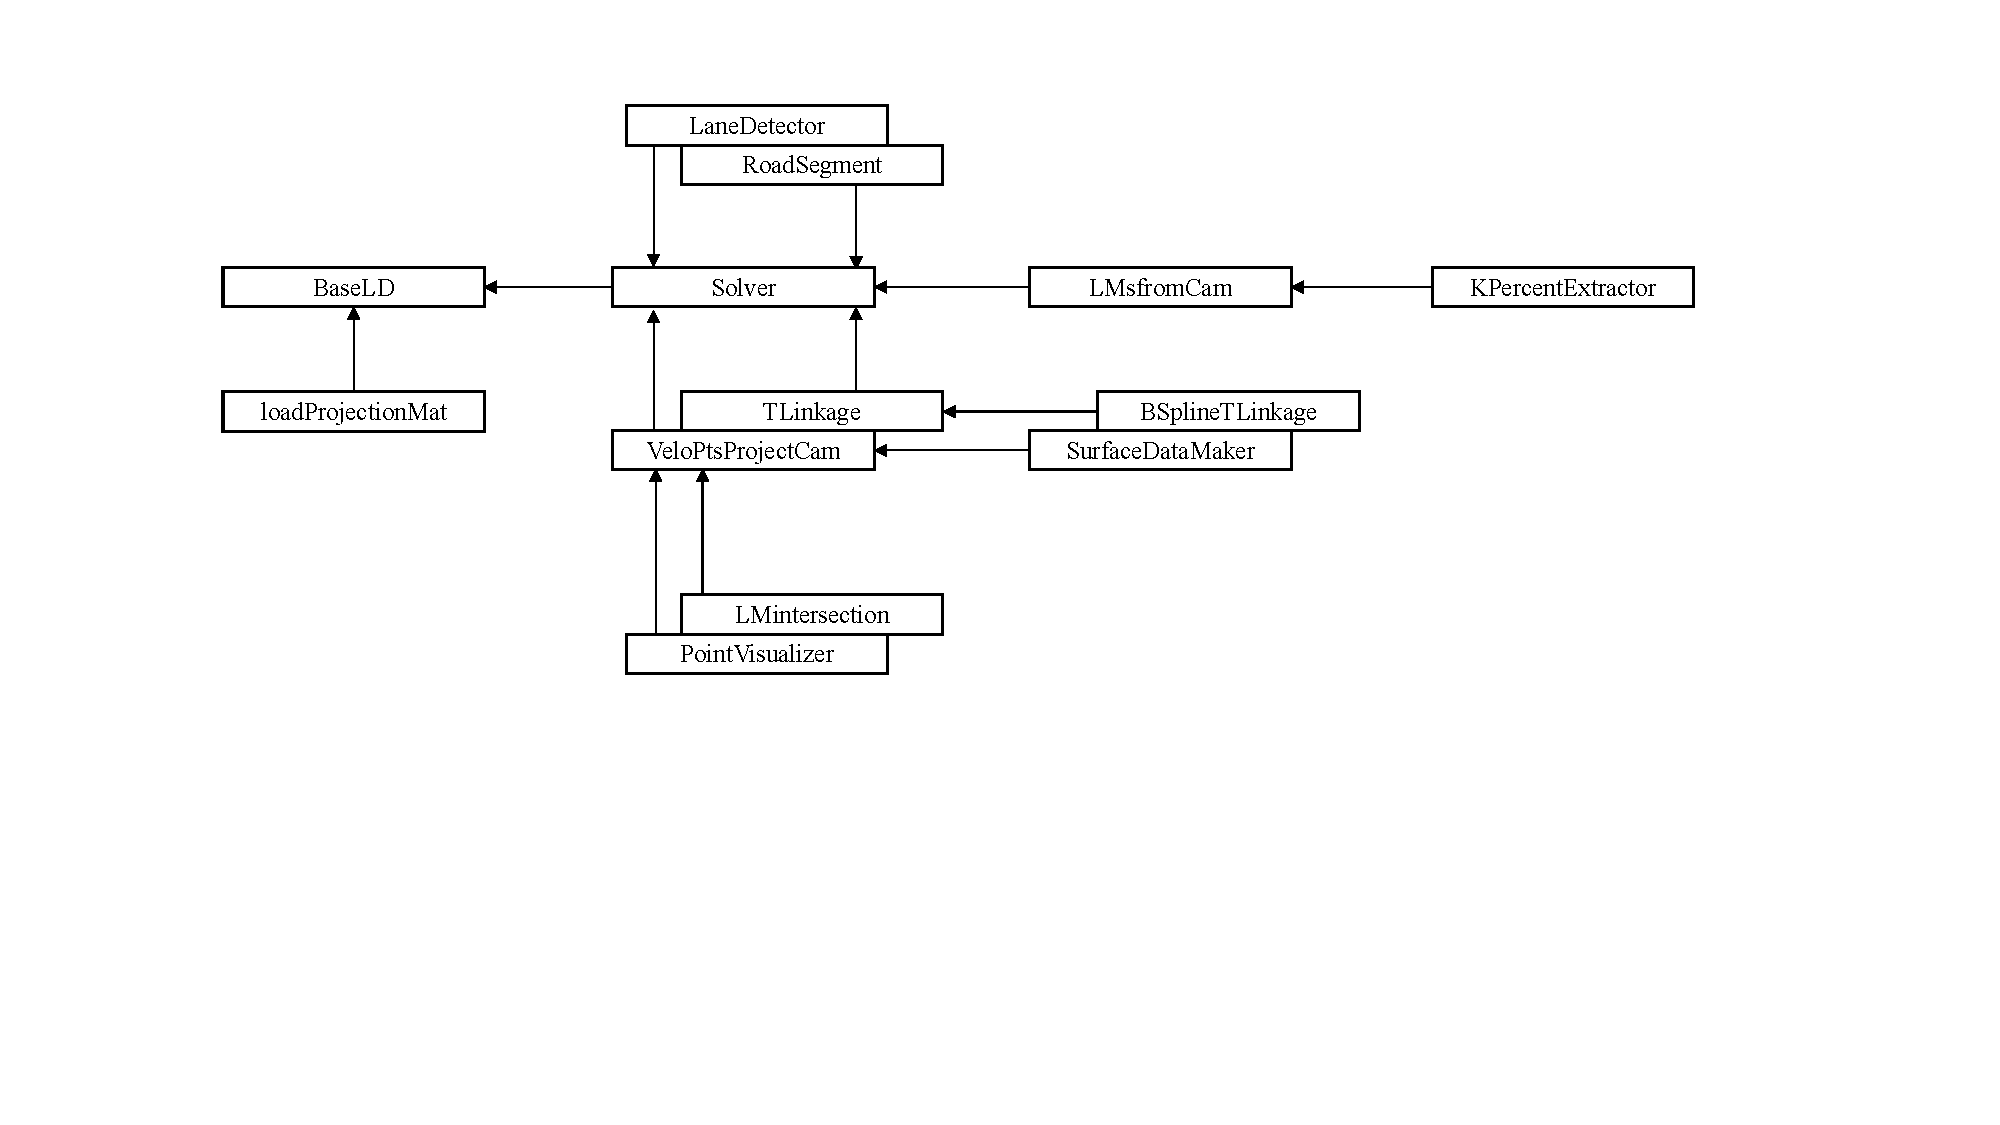
\includegraphics[width=0.9\columnwidth, viewport= 103 213 816 495, clip = true]{figure/classdiagrampptx.pdf}
	\caption{Class diagram for the proposed framework. The solid arrow indicates ``is-a'' relationship.}
	\label{fig:classes}
\end{figure}

We refer to the class diagram in Fig.\ref{fig:classes}  to visualize the interplay of the framework. 
It mainly contains the following classes,
\begin{itemize}
	\item \verb+loadProjectionMat+ load KITTI's \verb+calib_velo_to_cam.txt+ and  \verb+calib_cam_to_cam.txt+ to get the projection matrix $\mathbf{P}$ from LIDAR to camera. The user/reader is required to change the \verb+Parameter.xml+ to locate those files.
	\item \verb+RoadSegment+ obtain the road surface image mask \cite{zhao2017icnet} from color images through ICNet \cite{zhao2017icnet}. It loads  the model file \verb+icnet_cityscapes_train_30k.caffemodel+ from the folder \verb+/model+ and the configuration file  \verb+icnet_cityscapes.prototxt+ in the folder\verb+/prototxt+.  Change the class constructor in class \verb+RoadSegment+ if you want to deploy different models and configuration files. 
	\item \verb+LMsfromCam+ detect lane marking pixels  and output  image mask for lane markings from images. The user/reader is required to change the \verb+Parameter.xml+ in the source code to locate the images. 
	\item \verb+VeloPtsProjectCam+ project 3D LIDAR point cloud into the image using  $\mathbf{P}$ from \verb+loadProjectionMat+. 
	\item \verb+LMintersection+ intersect lane marking points from image and the corresponding LIDAR scan with the same timestamps at LIDAR system coordinate in order to determine the boundary models. 
	\item \verb+SurfaceDataMaker+ display the projected LIDAR points belonged to the road surface on image by using the image mask from class \verb+RoadSegment+. 
	\item \verb+KPercentExtractor+ extract lane markings from image and refine the results through vanishing point detection.
	\item \verb+TLinkage+  a multi-model fitting approach.
	\item \verb+BSplineTLinkage+ B-spline lane boundary curve model.
	\item \verb+LaneDetector+ detect lane markings from the image and LIDAR scan,  obtain the lane boundary models, and compute the lane quality metrics. 
\end{itemize}






For sample source data and experimental results, please look into the \verb+data+ folder. This documentation is by no means complete, but it is intended to help the user browsing the C++ code.


\subsection{Configuration File}

The framework requires two command line arguments (see \verb+main.cpp+), and the second argument is the configuration file, i.e., \verb+Parameters.xml+, which contains the environment settings for the whole framework. Through the configuration file, the user/reader can choose the folders to read source data, set threshold values for each classes, and output experimental results. Several important parameters are provided below,
%In \verb+Parameters.xml+, are declared to locate the image sequence, LIDAR scan, calibration file and the set of images that the user/reader is specially interested in and want to test.
\begin{itemize}
	\item \verb+dataRoot+ the path to the folder that contains a sequence of  RGB images collected from the front-view camera. 
	\item  \verb+dataFile+ the path to the file that contains a set of image's name that the user/reader is interested to get the quality metrics or the lane models. 
	\item \verb+veloRoot+ the path to the folder that contains a sequence of binary files, which contains a set of LIDAR points. 
	\item \verb+segImgPrefix+  the name prefix for segmented road surface image mask for \verb+RoadSegment+ in Fig.\ref{fig:classes}. The image mask, a binary image, indicates the road surface pixel coordinates in the  image. 
	\item \verb+overlayedRoot+  the directory to store the color images by overlaying the image mask with the original image for visualization. 
	\item \verb+refinedRoot+ the directory to store the lane marking's image mask.
	\item \verb+refinedImgPrefix+ the name prefix for the lane marking's image mask.
	\item \verb+minSamples+ the minimum number of 3D LIDAR points for the B-spline lane boundary models.
	\item \verb+ratiosFile+ the path to the file to store the lane quality metrics.	
	\item \verb+modelFile+ the path to the file to store the B-spline lane boundary curve mode.
\end{itemize} 

The framework loads the configuration file, and parses the parameter setting into different classes for initialization (see Listing \ref{ll::maincpp}). 

\subsection{Functionality Selection}

Through pugixml library \cite{kapoulkine2012pugixml}, we provide a flexible easy-to-use structure to execute different functionalities by changing the ``solver'''s name in the configuration file (see Listing \ref{ll::solver}). 
\begin{lstlisting}[float, label=ll::solver, caption = Change the configuration file to select the functionality.]
<?xml version="1.0" encoding="UTF-8"?>
	<Document>
		<Solvers>
		......
			<LaneDetector 
			......
				lassAsses="false"
			......
			/>
		......
		<!--change the solver to execute the functional block-->
		<Main solver="LaneDetector" debug="true"/>
</Document>
\end{lstlisting}
Replace the ``solver'''s name to accomplish the target task without repeatably executing all the other functionalities. It greatly decreases the debugging time and increase the codding efficiency.  The only requirement is that the user/reader needs to store all the intermediate results from all the previous steps.  For example, the  \verb+RoadSegment+ provides road surface image mask for \verb+LMsfromCam+, which is required to be saved as input for the class \verb+LMsfromCam+. The \verb+main.cpp+ parses the ``solver'''s name, select the classes listed in Listing \ref{ll::maincpp}, and execute the corresponding one. We suggest to follow the steps, \verb+RoadSegment+ \verb+->+ \verb+KPercentExtractor+ \verb+->+\verb+LMsintersection+ \verb+->+\verb+BSplineTLinkage+, to get the intermediate results such as road mask, lane marking points in the LIDAR scan, and lane boundary model. The class \verb+LaneDetector+  will execute all the above steps. For complete analysis, replace the ``solver'''s name with ``\verb+LaneDetector+" like Listing \ref{ll::solver} and perform  road surface segmentation to lane quality metric computation. 

The current framework provides the capabilities to switch between lane quality assessment mode and lane detection mode. If \verb+lassAsses="false"+ in Listing \ref{ll::solver},  the framework will stop  computing the quality metrics. The user/reader decides the way of exploiting the framework and has the freedom to choose the functionality according to different application scenarios. 

We also have a user-defined debug mode (see \verb+m_debug+ in class \verb+BaseLD+) to provide additional runtime information of the framework. Change \verb+debug ="true"+ in Listing \ref{ll::solver} to \verb+debug ="false"+ to stop the user-defined debug mode. 

\begin{lstlisting}[float,  label=ll::maincpp, caption =  Parse Parameter.xml to execute  different functionality in main.cpp.]
int main(int argc, char *argv[]) {
	if (argc != 2)
	throw runtime_error("ERROR: xml file is expected!");
	
	pugi::xml_document xml;
	pugi::xml_parse_result status = xml.load_file(argv[1]);
	if (!status)
	throw runtime_error(string("xml error") + status.description());
	
	string solver = xml.document_element().child("Main").attribute("solver").as_string();
	std::unique_ptr<LD::Solver> solverPtr = nullptr;
	
	if (boost::iequals(solver, "RoadSegment"))
		solverPtr = std::make_unique<RoadSegment>(argv[1]);
	else if (boost::iequals(solver, "KPercentExtractor"))
		solverPtr = std::make_unique<KPercentExtractor>(argv[1]);
	else if (boost::iequals(solver, "LMsintersection"))
		solverPtr = std::make_unique<LMsintersection>(argv[1]);
	else if (boost::iequals(solver, "BSplineTLinkage"))
		solverPtr = std::make_unique<BSplineTLinkage>(argv[1]);
	else if (boost::iequals(solver, "Line3DTLinkage"))
		solverPtr = std::make_unique<Line3DTLinkage>(argv[1]);
	else if (boost::iequals(solver, "LaneDetector"))
		solverPtr = std::make_unique<LaneDetector>(argv[1]);
	else
		throw runtime_error("No such solver implemented: " + solver);
	
	solverPtr->Run();
	
	return 0;
}
\end{lstlisting}

\subsection{Error Capture}
If the current lane that the autonomous vehicle is driving on does not have any lane markings, the system  outputs \verb+WARNING: Could not find enough samples!+ in the \verb+ratio.txt+ file.  Other possible runtime errors are also captured as well.  Please look into class \verb+LaneDetector+ for detailed implementation.


\section{Tools}

\subsection{Compatibility with the Velodyne LIDAR System}

For the \verb+pcap+ file or  live stream from Velodyne 16/32E/64E, please refer to the folder \verb+3rdParty/pcap2kitti+ to convert to the binary files. For \verb+pcap+ file, run \verb+pcap2kitti+ \verb+filename.pcap+ and obtain binary files frame by frame. For live stream output from the Velodyne, change the IP address and port number in \verb+pcap2kitti.cpp+. Noted we provide standalone package to convert Velodyne output to KITTI's binary format. It is not integrated with the lane quality assessment framework for the purpose of convenience of the usage. If complete integration is required, change the function  \verb+ReadVeloData+ in  class \verb+VeloPtsProjectCam+. 

\subsection{Vanishing Point Detection}
We employ line segment detection \cite{von2012lsd} for vanishing point detection to refine lane marking detection results from the images. Detailed usage is in the  class \verb+KPercentExtractor+.

\subsection{Lane Boundary Model Compatibility}
We use T-linkage \cite{magri2014t}, a multi-model fitting approach, to obtain the lane boundary models. We apply cubic B-spline curve models into the T-linkage to get left and right lane boundaries. We also provide 3D line lane models in folder \verb+3rdParty/TLinkage+. To use the line models, simply change the ``solver'' name to \verb+Line3DTLinkage+  in the configuration file \verb+Parameters.xml+ (see Listing \ref{ll::solver}). 

\section{Contributors}
\begin{tabular}{lll}
	Dezhen Song       & Project Director, Concept Design              \\
	Binbin Li         & System Design, Primary Software Developer     \\
	Aaron Kingery     & Software Developer, Tester, and Documentation \\
	Aaron Angert      & Software Developer, Tester, and Documentation \\
	Ankit Ramchandani & Software Developer, Tester, and Documentation 
\end{tabular}




{\small
\bibliographystyle{unsrt}
\bibliography{doc.bib}}

\end{document}